\documentclass[a4paper]{standalone}

\usepackage{pgfplots}

\pgfplotsset{compat=1.3}

\begin{document}
\parindent=0pt
\parskip=20pt

\def\plots{
	\addplot+[domain=0:5] {x^2};
}

%\tracingmacros=2 \tracingcommands=2
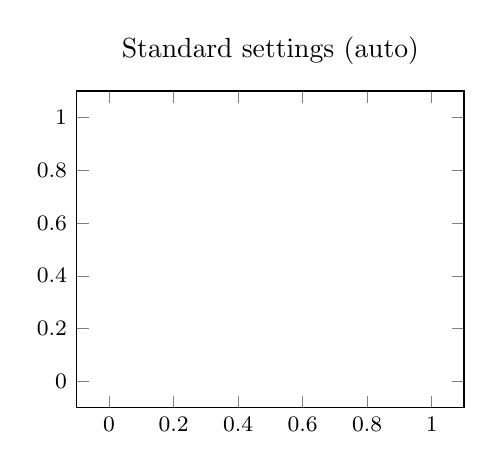
\begin{tikzpicture}
\begin{axis}[
	title=Standard settings (auto),
	small,
]
	\plots
\end{axis}
\end{tikzpicture}
\message{^^J^^JSecond picture ^^J^^J}%
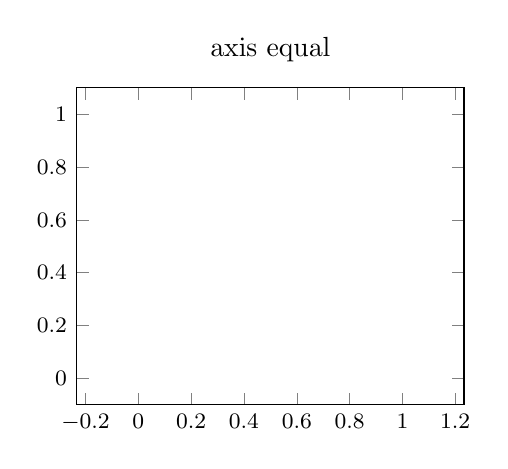
\begin{tikzpicture}
\begin{axis}[
	title=axis equal,
	axis equal,
	small]
    \plots
\end{axis}
\end{tikzpicture}

\message{^^J^^JThird picture ^^J^^J}%
\pgfplotsset{small,width=5cm,height=7cm}

\begin{tikzpicture}
\begin{axis}[
	title=Standard settings (auto),
	%small,
]
    \plots
\end{axis}
\end{tikzpicture}
\message{^^J^^JFourthh picture ^^J^^J}%
\begin{tikzpicture}
\begin{axis}[
	title=axis equal,
	axis equal,
	% this fixes it:
	%scale uniformly strategy=change horizontal limits,
	%small,
]
    \plots
\end{axis}
\end{tikzpicture}
\end{document}

